\section{Probenherstellung und Messmethoden}\label{sec:messmethoden}

\subsection{Pulsed Laser Deposition}\label{subsec:pld}
Die erste Aufgabe des Versuchs besteht darin, \heo-Dünnfilme herzustellen, die eine Dicke von wenigen hundert
Nanometern aufweisen.
Um das zu erreichen, verwendet man Pulsed Laser Deposition (PLD).
Dafür wird ein Laserstrahl auf einen Festkörper, dem Target, ausgerichtet, welches beginnt zu
verdampfen und sich auf ein Substrat absetzt.
Im Folgenden soll dieser Mechanismus genauer beschrieben werden.

\subsubsection{Aufbau}
Ein PLD-System besteht aus einem Laser, einer Vakuumkammer und den darin befindlichen Komponenten.

\paragraph{Laser}
Der Laser (Light Amplification by Stimulated Emission of Radiation) bildet das Herzstück des gesamten PLD Prozesses.
In diesem wechselwirken Gasatome mit einem elektrischen Feld, sodass sie in einen angeregten Zustand übergehen.
Anschließend wird das Prinzip der stimulierten Emission genutzt.
Das angeregte Elektron verweilt vergleichsweise lange im angeregten Zustand und relaxiert durch ein
weiteres Photon von außerhalb zurück in den Grundzustand.
Bemerkenswerterweise haben beide Photonen dadurch identische Eigenschaften wie Phase, Amplitude und Frequenz.
Somit wird ein Lichtstrahl erzeugt, der sich durch Kohärenz und Monochromatizität auszeichnet.
Durch einen Satz von Spiegeln im Inneren des Lasers kann der Strahl durch die Stimulierung weiterer Gasatome
verstärkt werden.
Abschließend wird der Strahl durch ein halbdurchlässiges Fenster emittiert. \autocite[2296-2297]{pld}

\paragraph{Vakuumkammer}
Der Laserstrahl wird anschließend durch ein Fenster in die Vakuumkammer, dem nächsten Bestandteil des PLD Prozesses,
geleitet.
In dieser kann mithilfe von Vor- und Turbomolekularpumpen ein Vakuum in der Größenordnung von
\qty{e-4}{\milli\bar} erzeugt werden.
Zusätzlich können auch Hintergrundgase wie Sauerstoff, Stickstoff oder Argon in die Kammer eingelassen werden.
Das Vakuumlevel beeinflusst einerseits die Zusammensetzung der Plasmawolke, andererseits auch die
Zeit, die benötigt wird, um eine einzelne Schicht von Adsorbaten auf dem Substrat abzuscheiden.
Eine Reduktion des Drucks führt damit zu einer stabileren Umgebung für die Dünnfilmabscheidung.\autocite[2297-2298]{pld}

\paragraph{Targethalter, Substrathalter, Heizer}
In der Vakuumkammer ist ein scheibenförmiges Target an einer Halterung montiert, welches aus dem Material besteht, aus
dem der Dünnfilm hergestellt werden soll.
Da das Target durch den Laserstrahl nur an einer kleinen Stelle erhitzt wird, ist es notwendig,
dass sich das Target relativ zum Laserstrahl bewegt, um eine gleichmäßige Abtragung zu gewährleisten.
Dafür reicht eine einfache Rotation aus.

Hinzu kommt ein Substrathalter, auf dem das Substrat montiert wird.
Dieses kann durch einen Widerstandsheizer auf eine Temperatur von bis zu \qty{1000}{\celsius} beziehungsweise
mithilfe eines Laserheizers auf circa \qty{1500}{\celsius} erhitzt werden.
Das Substrat selbst hat üblicherweise die Maße von circa \qty{10}{\milli\meter\squared}.\autocite[2299]{pld}

\subsubsection{Abscheidungsprozess}
Mithilfe der oben genannten Komponenten kann der Abscheidungsprozess durchgeführt werden.
Die Laserphotonen treffen auf das Target und regen dort Elektronen an.
Diese erfahren einen Intraband-Übergang, wodurch sie in einen angeregten Zustand übergehen.
Durch die Elektron-Phonon-Wechselwirkung relaxiert das Elektron und gibt dabei Energie in Form von Phononen ab.
Dies führt zur Erhitzung des Targets, welche nicht nur an der Oberfläche, sondern auch im Inneren stattfindet.
Durch die hohe Temperatur beginnt das Target zu Verdampfen.

Auch die verdampften Konstituenten des Targets wechselwirken mit den Laserphotonen.
Durch Photoionisation werden Elektronen herausgelöst, sodass eine Plasmawolke entsteht.
Diese breitet sich in der Vakuumkammer in Richtung Substrat aus und beginnt sich auf dem diesem abzusetzen.
Durch Adsorptionsprozesse beginnt die Bildung eines Dünnfilms.\autocite[2299-2301]{pld}

\subsection{XRD}\label{subsec:xrd}
Nachdem die Dünnfilme hergestellt wurden, ist der nächste Schritt, ihre Struktur zu charakterisieren.
Zwischen Dünnfilmen und ihren korrespondierenden Massivkörpern existieren signifikante Unterschiede.
Diese resultieren vorrangig aus dem Verhältnis von Oberfläche zu Volumen, sowie den jeweiligen
Wachstumsbedingungen, wie Temperatur, Druck und Substrat.
Sie zeigen sich beispielsweise in der Qualität der Kristallinität, sowie in Kompositionsgradienten.
Da Proben mit unterschiedlichen Wachstumsbedingungen hergestellt wurden und deren Eigenschaften dadurch
maßgeblich beeinflusst werden, ist es notwendig, die Kristallinität der Dünnfilme zu charakterisieren.
Röntgendiffraktometrie (XRD, engl. \textit{X-Ray diffraction}) ist eine weit verbreitete Methode, um die
Kristallstruktur von Dünnfilmen zu bestimmen.
Dabei wird ein Röntgendiffraktometer verwendet.

\subsubsection{Röntgendiffraktometer}
Das Röntgendiffraktometer besteht aus fünf Hauptkomponenten: Röntgenquelle und Detektor, Ein- und Ausfallsoptik,
sowie dem Goniometer.
Zusätzlich ist das Diffraktometer durch eine Strahlungsschutzverkleidung abgeschirmt und mit einer Steuerungssoftware
verbunden.
Im Folgenden werden die einzelnen Komponenten näher erläutert.

\paragraph{Röntgenquelle}
Die Röntgenstrahlen werden in einer Röntgenröhre erzeugt.
In dieser werden Elektronen aus einer Wolfram-Glühkathode emittiert und durch das elektrische Feld auf eine Anode
beschleunigt.
Die Anode besteht meist aus hochreinem Kupfer.
Stromstärke und Beschleunigungsspannung der Röntgenröhre müssen so gewählt werden, dass die Energie beim Auftreffen der
Elektronen auf die Anode ausreicht, um die gebundenen Elektronen der Atome auf das nächsthöhere Energieniveau anzuregen.
Aufgrund der daraus resultierende Wärme muss die Anode ständig wassergekühlt werden.
Im hauseigenen Röntgendiffraktometer wird eine Beschleunigungsspannung von \qty{40}{\kilo\volt} und eine Stromstärke
von \qty{40}{\milli\ampere} verwendet.

Nach der Kollision zwischen Kupferatom und Elektron relaxiert das Elektron unter Bildung eines Röntgenphotons.
Man erhält ein Spektrum, welches durch die charakteristische Strahlung der Anode sowie durch Bremsstrahlung
geprägt ist.
Die charakteristische Strahlung wird vorrangig durch die K-Linien, insbesondere $K_{\alpha_1}$, $K_{\alpha_2}$
und K$_{\beta}$, dominiert.
Da $K_{\alpha_1}$ und $K_{\alpha_2}$ energetisch sehr nahe beieinander liegen, können sie nicht immer einzeln
aufgelöst werden.
Die $K_{\beta}$ Strahlung ist größtenteils unerwünscht und kann durch geeignete Filter unterdrückt werden.

Die Wolfram-Glühkathode emittiert unerwünschterweise nicht nur Elektronen, sondern auch Wolfram-Atome in kleinen Mengen.
Über längere Zeiträume führt dies zu einer nicht mehr zu vernachlässigenden Kontamination der Anode.
Dadurch können bei Elektronenstößen auch Wolfram-Atome angeregt werden, was zu einer zusätzlichen Wellenlänge im
Spektrum führt
In den späteren Messergebnissen sind diese Beiträge erkennbar.
Abschließend gelangen die Röntgenstrahlen durch ein Berylliumfenster in die Einfallsoptik.

\paragraph{Goniometer}
Das Goniometer ist die mechanische Komponente des Röntgendiffraktometers.
Es besteht aus mehreren Drehachsen, die es ermöglichen, die Probe in unterschiedlichsten Winkeln auszurichten.
Nach der Braggschen Beugungstheorie ergeben sich konstruktive Interferenzen an denjenigen Winkeln, die der
Bragg-Bedingung genügen.
Existieren Möglichkeit, die Winkel für Quelle und Detektor zu variieren, kann diese Interferenz beobachtet werden.
Im Allgemeinen ist die Röntgenquelle jedoch fest, eine äquivalente Drehung von Probe und Detektor ist deshalb gängig.
In der einfachsten Betrachtungsweise muss das Goniometer also den Winkel zwischen Probe und Quelle ($\omega$) und dem
Winkel zwischen Probe und Detektor ($2\theta$) einstellen können.
Diese Freiheit reicht zwar für Pulverproben, jedoch nicht für Dünnfilme.
Zwar kann man mit beiden Freiheitsgraden Messungen durchführen, welche die out-of-plane Orientierung charakterisieren,
jedoch ist es nicht möglich, die in-plane Orientierung zu bestimmen.
Dafür werden weitere Achsen, wie $\varphi$ und $\chi$, benötigt.
Eine Konstruktion mit den vier Achsen wird Euler-Wiege genannt.

\paragraph{Ein- und Ausfallsoptik}
Es existieren zwei primäre Möglichkeiten, um den Strahlengang zwischen Quelle, Probe und Detektor zu modifizieren:
Bragg-Brentano-Geometrie und parallele Geometrie.
In der Bragg-Brentano-Geometrie wird ein hochintensiver, divergierender Röntgenstrahl auf die Probe gerichtet,
welcher unter Ausnutzung bestimmter Geometrien zurück auf den Detektor fokussiert werden kann.
Aufgrund der Divergenz des Strahls ist diese Methode fehleranfällig und gerade für $\varphi$ und $\omega$ scans
ist eine Parallelstrahloptik, wie in \cref{fig:xrd_parallel} gezeigt, von Vorteil.
\begin{figure}
    \centering
    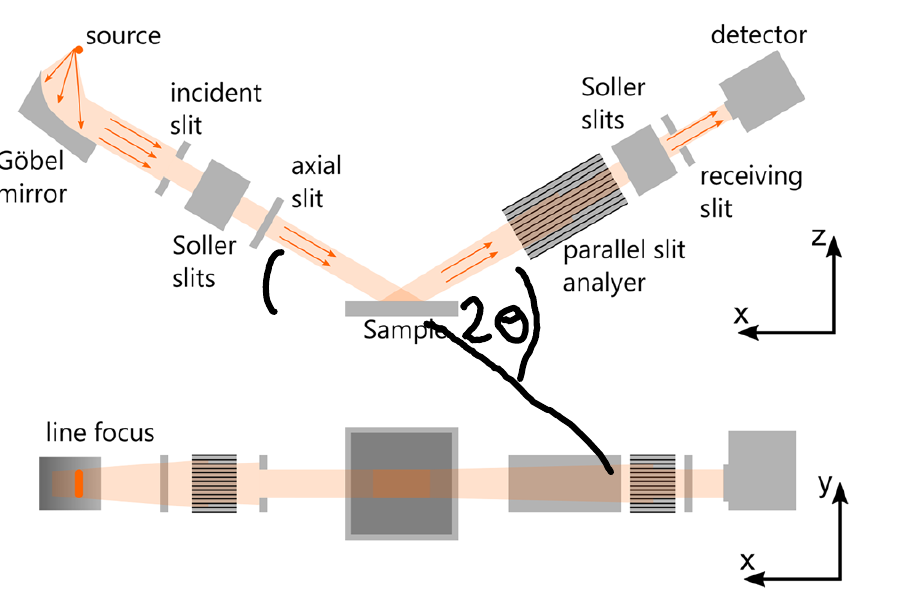
\includegraphics[width=0.6\textwidth]{../assets/messmethoden/xrd/paralleloptik}
    \caption{Aufbau der Parallelstrahloptik \imcitetwo[146]{btb-xrd}}
    \label{fig:xrd_parallel}
\end{figure}
Die aus der Quelle austretenden divergierenden Strahlen werden durch einen Göbel-Spiegel
parallelisiert und durchlaufen anschließend einen Eingangs- und Axialspalt, die den Winkelbereich
festlegen.
Dazwischen liegt ein Soller Spalt, der die Divergenz in axialer Richtung begrenzt, da diese
nicht durch den Göbel-Spiegel eliminiert werden kann.
Anschließend reflektiert der Strahl an der Probe und gelangt über weitere Spalte zum Detektor.

\paragraph{Detektor}
Der Röntgendetektor dient dazu, die Intensität der reflektierten Röntgenstrahlen zu messen und
in elektrische Signale umzuwandeln.
Im hauseigenen Röntgendiffraktometer wird ein Halbleiterdetektor verwendet
Die Grundidee eines Halbleiterdetektors ist, das Material durch Photonen zu ionisieren und dabei freie Ladungsträger zu
erzeugen.
Diese werden über ein elektrisches Feld extrahiert und elektronisch gezählt.
Durch die matrixartige Anordnung einzelner Halbleiterzellen kann die Intensität in Abhängigkeit der Position bestimmt
werden.
Somit können unterschiedliche Detektormodi realisiert werden, wie 0D Punktdetektion,
1D Linien- oder 2D Flächendetektion.
Wichtig ist, dass die maximale Zählrate des Detektors nicht überschritten wird.
Das führt zu nicht linearen Antworten und kann den Sensor beschädigen.
Um das zu vermeiden, können Filter und Attenuatoren verwendet werden.

\subsubsection{Scanmethoden}
Durch den hohen Freiheitsgrad des Goniometers können unterschiedliche Scanmethoden realisiert werden.
Diejenigen, die in dieser Arbeit verwendet wurden, sind im Folgenden beschrieben.

\paragraph{$2\theta/\omega$ scan}
Ein $2\theta/\omega$ scan ist eine einfache Methode, um die Kristallstruktur von Dünnfilmen zu bestimmen
und bildet die Grundlage für weitere Messungen.
Die Probe wird auf den Probenhalter montiert und in das Goniometer eingesetzt.
Der Winkel zwischen Probenoberfläche und Quelle wird als $\omega$ und der Winkel zwischen Probenoberfläche und Detektor
als $2\theta$ bezeichnet.
Als Anfangsbedingung legt man Messdauer und ein Intervall für $\omega$ fest und startet die Messung.
Nun fahren Goniometer und Detektor über den angegebenen Winkelbereich mit der Bedingung $\omega = \theta$.
Als Ausgabe bekommt man ein Intensitätsprofil in Abhängigkeit von $2\theta$, in denen im Idealfall charakteristische
Peaks erkennbar sind.
Diese Peaks entstammen der Bragg-Reflexion von Kristallebenen, die parallel zur Probenoberfläche liegen.
Kennt man die Wellenlänge der Röntgenstrahlung, so kann mam mithilfe des Peaks den Gitterabstand bestimmen.
Somit ist es möglich, Rückschlüsse auf die vorhandenen Kristallstrukturen im Dünnfilm zu ziehen.

\paragraph{$\omega$ scan}

\paragraph{$\varphi$ scan}
%%TODO

\subsection{Rasterkraftmikroskopie}\label{subsec:afm}
Nachdem die Kristallinität mithilfe von XRD untersucht wurde, kann durch Rasterkraftmikroskopie (AFM, engl.
\textit{Atomic Force Microscopy}) die Oberflächenstruktur der Dünnfilme charakterisiert werden.
Das Rasterkraftmikroskop ist ein hochpräzises Messinstrument zum Erfassen von Oberflächenstrukturen.
Anders als bei Licht- oder Elektronenmikroskopie wird hierbei eine mechanische Funktionsweise umgesetzt.
Dabei fährt eine Messapparatur, der Cantilever, rasterweise über eine Oberfläche und tastet diese ab.
Die auf den Cantilever wirkenden atomaren oder magnetischen Kräfte werden gemessen, woraus eine Topographiekarte der
Oberfläche erstellt wird.

\subsubsection{Schematischer Aufbau und Funktionsweise}
\begin{figure}
    \centering
    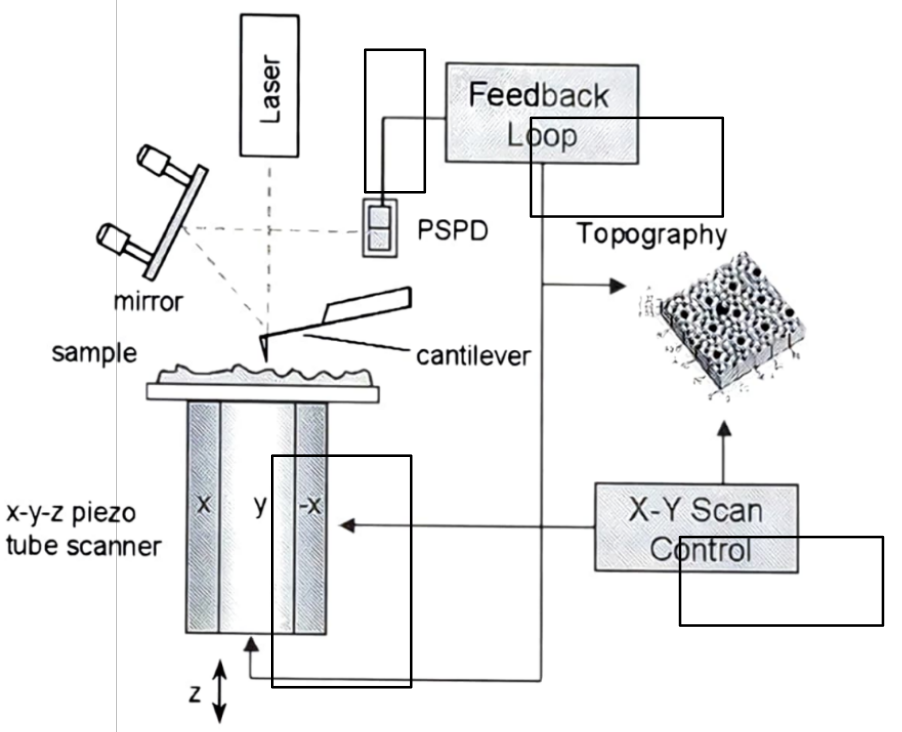
\includegraphics[width=0.6\textwidth]{../assets/messmethoden/afm/01_aufbau}
    \caption{Schematischer Aufbau eines Rasterkraftmikroskops. \imcitetwo[12]{afm-handbuch}}
    \label{fig:afm_aufbau}
\end{figure}
Die grundlegende Funktionsweise ist in \cref{fig:afm_aufbau} dargestellt.
Markierung 1 zeigt den Cantilever, der mit einer Messspitze mit Dimensionen im Nanometerbereich ausgestattet ist.
Fährt diese über die Probe, so wirken Kräfte auf die Spitze, welche den Cantilever auslenken.
Diese Auslenkung wird mittels eines Ablenkungserkennungssystems, Markierung 2, ausgewertet.
Die gemessene Auslenkung wird an das Feedback System übergeben, was Markierung 3 zeigt.
Basierend auf dem gewählten Betriebsmodus wird versucht, die gemessene Kraft oder Amplitude konstant zu halten.
Mithilfe dieser Regulation wird ein Korrektursignal ausgegeben, welches die Position des Cantilevers anpasst.
Dies geschieht mithilfe von Piezoelementen, wodurch der Cantilever in $x$, $y$ oder $z$-Richtung bewegt werden kann,
siehe Markierung 4.
Die z-Position des Cantilevers wird aufgezeichnet und als Topographiesignal am Computer ausgewertet, siehe Markierung 5.
Im Folgenden werden die einzelnen Komponenten näher erläutert.\autocite[8-10]{afm-buch}

\subsubsection{Interaktion zwischen Probe und Spitze}
Zuerst wird die Wechselwirkung zwischen Cantileverspitze und Probe betrachtet.
Die auf die Spitze wirkende Gesamtkraft setzt sich aus verschiedenen Komponenten zusammen.
Der wichtigste und weitreichendste Beitrag entspringt der Van-der-Waals Wechselwirkung.
Diese ist eine attraktive Kraft, welche durch spontane Formationen fluktuierender Dipole entsteht.
Für einzelne Edelgasatome lässt sich das Potential der Wechselwirkungen durch
$U_{\mathrm{vdW}}\propto-r^{-6}$ annähern.
Obwohl diese Näherung für einzelne Atome gilt, kann sie durch Integration über das Probe-Spitze System genutzt
werden, um es zu beschreiben.
Für Distanzen zwischen Probe und Spitze größer als \qty{1}{\nano\meter} ist die Van-der-Waals Wechselwirkung
dominierend.

Für kleinere Distanzen müssen zwei weitere Interaktionen berücksichtigt werden.
Überlappen die äußeren Elektronenhüllen von Proben- und Spitzenatomen, so können chemische Bindungen entstehen, welche
eine attraktive oder repulsive Kraft hervorrufen.
Betrachtet man noch kleinere Distanzen, so wird die Pauli-Abstoßung zwischen den Elektronen der Atome relevant.
Da die geschlossenen Elektronenschalen der Atome nicht überlappen können, müssen die zusätzlichen Elektronen auf ein
höheres Energieniveau gehoben werden.
Dadurch entsteht eine effektive repulsive Kraft.

Obwohl das System quantenmechanisch präzise beschrieben werden kann, ist die Lösung für solch komplexe Systeme
nicht trivial.
Aus diesem Grund werden Modellpotentiale genutzt, die die Interaktionen zwischen Probe und Spitze approximieren.
Ein beliebtes ist das Lennard-Jones-Potential, welches sowohl die Van-der-Waals Wechselwirkung als auch die repulsiven
Anteile berücksichtigt.
\begin{equation*}
    U_{\mathrm{LJ}}=4U_{0}\left[ \left( \frac{R_{\mathrm{a}}}{r} \right)^{12} -\left( \frac{R_{\mathrm{a}}}{r}
    \right)^{6}\right]
\end{equation*}
Hierbei ist $U_{0}$ die Tiefe des Potentials, $R_{\mathrm{a}}$ der Gleichgewichtsabstand und $r$ der Abstand zwischen
den Atomen.
Auch wenn das Lennard-Jones-Potential für atomare Wechselwirkungen entwickelt wurde, erklärt es die relevanten
Kräfte zwischen Probe und Spitze. \autocite[161-164]{afm-buch}

\subsubsection{Auslenkungserkennungssystem}
\begin{figure}
    \centering
    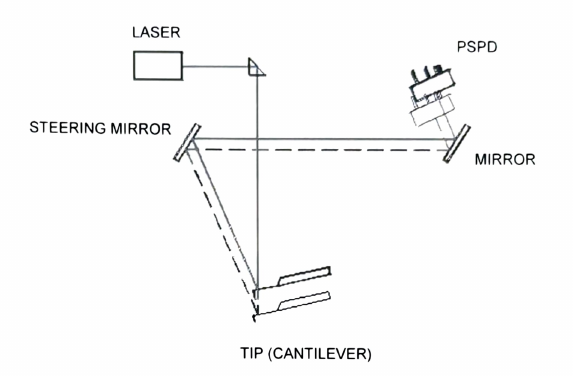
\includegraphics[width=0.6\textwidth]{../assets/messmethoden/afm/02_beam}
    \caption{Schematischer Aufbau eines Auslenkungserkennungssystems. \imcitetwo[17]{afm-handbuch}}
    \label{fig:afm-beam}
\end{figure}
Nachdem der Cantilever durch die Wechselwirkungskräfte ausgelenkt wurde, muss diese Auslenkung gemessen werden.
Das System ist in \cref{fig:afm-beam} dargestellt.
Ein Laserstrahl wird aus einer Laserdiode emittiert und auf die Rückseite des Cantilevers gerichtet.
Dieser besitzt eine reflektierende Rückseite, sodass der Strahl am Cantilever zum beweglichen Spiegel reflektiert wird.
Über diesen Lässt sich die Potition des Strahls auf den folgenden Spiegel steuern.
Der letzte Spiegel reflektiert den Strahl auf einen positionsabhängigen Photodetektor.
Dieser besitzt vier Segmente, die die Intensität des reflektierten Strahls messen.
Im unausgelenkten Zustand, muss der bewegliche Spiegel so eingestellt werden, dass der Strahl mittig auf die vier
Segmente trifft.
Kommt es zur Auslenkung, ändert sich der Winkel des Cantilevers und damit auch die Position des Strahls auf dem
Photodetektor.
Über die vier Segmente kann die Auslenkung und Torsion des Cantilevers bestimmt werden.

\subsubsection{Feedback Controller}
Damit eine möglichst genaue Topografiekarte aufgezeichnet werden kann, ist ein schnelles und präzises Regelsystem von
großer Bedeutung.
Ziel ist es, eine vorgegebene Kenngröße möglichst konstant zu halten, beispielsweise die Auslenkung des Cantilevers.
Dafür wird ein geschlossenes Regelkreissystem verwendet, welches in \cref{fig:afm_controller} dargestellt ist.
Der Ausgabewert des Systems $x(t)$, beispielsweise die Cantileverauslenkung, wird gemessen, zunächst mit dem
Sollwert $w$ verglichen und das Fehlersignal $e(t)=w-x(t)$ berechnet.
Dieses Fehlersignal wird an den Controller übergeben, der daraufhin ein Korrektursignal $y(t)$ ausgibt.
Dieses Korrektursignal wird vom System aufgenommen und intrinsisch verarbeitet, sodass der Ausgabewert $x(t)$ näher am
Sollwert $w$ liegt.\autocite[99-101]{afm-buch}
\begin{figure}
    \centering
    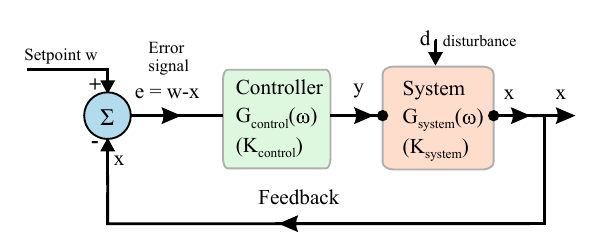
\includegraphics[width=0.6\textwidth]{../assets/messmethoden/afm/03_controller}
    \caption{Blockschaltbild eines Feedback-Controllers. \imcitetwo[14]{afm-buch}}
    \label{fig:afm_controller}
\end{figure}
Von besonderem Interesse ist nun die genaue Gestalt der Korrekturfunktion $y(t)$.
In der Regel wird diese durch einen Proportional-Integral-Controller (PI-Controller) realisiert und hat folgende Form:
\begin{equation*}
    y(t)=\underbrace{ K_{\mathrm{P}}(w-x(t)) }_{ \text{1. Proportional} }+\underbrace{ K_{\mathrm{I}}\int_{0}^{t}
        (w-x(\tau)) \, \mathrm{d}\tau }_{ \text{2. Integral} }
\end{equation*}\autocite[104-105]{afm-buch}

\paragraph{1. Proportional:}
Das Ausgabesignal wird Proportional zum Fehlersignal mit Proportionalitätskonstante $K_{\mathrm{P}}$ ausgegeben.
Dies ist die einfachste Art der Regulation, welche nur auf den aktuellen Zustand reagiert.
Der P-Regler zeichnet sich durch ein typisches Einschwingsignal aus, welches durch die Trägheit des Systems zustande
kommt.
Durch die Verzögerung zwischen Eingangssignal und Ausgangsreaktion des Systems entsteht oft eine Überreaktion,
diese Überschreitung ruft eine Gegenreaktion hervor, welche sich rekursiv zu einer Schwingung entwickelt.
Der größte Nachteil des P-Reglers ist, dass er nicht in der Lage ist, den Sollwert unter konstanter Störung
exakt zu erreichen.
Um diesen Nachteil zu beheben, wird zusätzlich ein I-Regler hinzugefügt.\autocite[101-102]{afm-buch}

\textbf{2. Integral:}
Der Integralanteil des Reglers reagiert auf die Summe der bisherigen Abweichungen mit Proportionalitätskonstante
$K_{\mathrm{I}}$.
Damit eliminiert er alle konstanten Störungen, die durch den P-Regler nicht beseitigt werden konnten.
Da das Integral des Fehlersignals über die Zeit gebildet wird, ist der I-Regler am Anfang sehr langsam.
In einigen Varianten wird nicht über das gesamte, sondern übern ein konstantes Zeitintervall integriert.
\autocite[102-104]{afm-buch}

Kombiniert man nun Proportional- und Integralregler, so können kurzzeitige Abweichungen durch den schnellen
P-Regler und langzeitige Abweichungen durch den langsamen I-Regler korrigiert werden.

\subsubsection{Piezoelemente und Positionierung}
Um den Cantilever in $z$, sowie die Probe in $xy$-Richtung zu bewegen, werden Piezoelemente verwendet.
Um diesen Mechanismus zu beschreiben, muss der Piezoeffekt betrachtet werden.
Setzt man Kristalle wie Quartz, die bestimmte Symmetrieeigenschaften aufweisen, unter mechanische Spannung,
so kann unter bestimmten Bedingungen elektrische Spannung induziert werden.
Diesen Effekt sieht man beispielsweise in Feuerzeugen.
Nun kann auch die Umkehrung des Effekts genutzt werden.
Legt man eine Spannung an einen Piezokristall an, kann dieser deformiert werden.
Für kleine Spannungen kann man so Deformationen im Bereich von \qty{0.1}{\nano\meter} erreichen.
\autocite[35-36]{afm-buch}

Um den Piezoeffekt zu nutzen, werden nun spezielle Metallbiegeelemente verwendet.
Das sind Metallblöcke, die sich in einer Richtung durch kleine Einschnitte federähnlich verformen lassen, während
sie in anderen Richtungen starr sind.
In diese können Piezoelemente eingebettet werden, sodass sich beim Anlegen einer Spannung der Block in eine Richtung
verformt und sich somit die Probe oder der Cantilever bewegt.
Wie in \cref{fig:afm_stage} dargestellt, lassen sich zwei orthogonale Piezoelemente kombinieren, um eine Bewegung in
$xy$-Richtung zu erreichen.
\begin{figure}
    \centering
    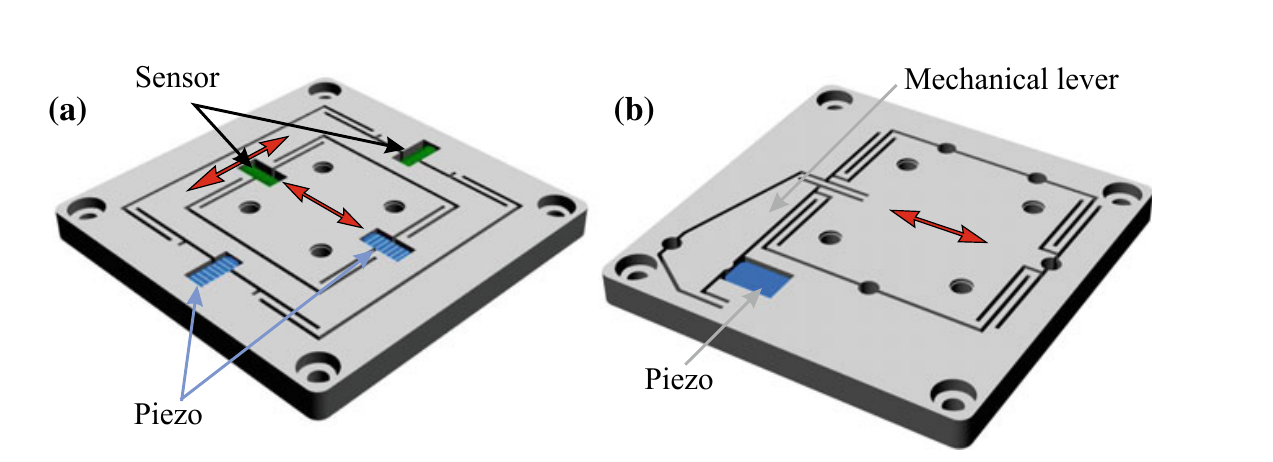
\includegraphics[width=0.6\textwidth]{../assets/messmethoden/afm/04_stage}
    \caption{Aufbau eines Biegeelements. \imcitetwo[74]{afm-buch}}
    \label{fig:afm_stage}
\end{figure}
\cref{fig:afm_aufbau} zeigt, zeigt eine Grobpositionsbühne, die
mithilfe von Stellschrauben motorisiert gesteuert wird.
Die Feinpositionierung und die Scanbewegung erfolgt dann mit den darauf montierten Piezo-Biegeelementen.
Der Cantilever samt Detektor wird unterhalb eines Piezoelements montiert, sodass er in $z$-Richtung bewegt werden kann.
\autocite[79-80]{afm-buch}

\subsubsection{Betriebsmodi}
Das Rasterkraftmikroskop verfügt über unterschiedliche Betriebsmodi.
In der vorliegenden Arbeit wurde im statischen Kontaktmodus verwendet, um die Oberflächenstruktur zu erfassen.
Dabei wird die Probe in $xy$-Richtung bewegt, während die Spitze des Cantilevers einen so kleinen Abstand zur Probe hat,
dass die repulsiven Kräfte dominieren.
Diese bewirken eine Auslenkung $\Delta z$ des Cantilevers, welche durch das Erkennungssystem aufgezeichnet wird.
Mithilfe eines \textit{setpoint}-Parameters wird eine konstante Auslenkung festgelegt, die vom Feedback-System
eingehalten wird.
Scannt man über eine Erhöhung, so ändert sich die Auslenkung und das Feedback-System versucht, den Cantilever erneut
auszurichten, indem es die Höhe anpasst.
Dadurch entsteht eine Topografiekarte der Oberfläche.
Dadurch, dass sich die Spitze in stetigem Kontakt mit der Oberfläche befindet, müssen die Wechselwirkungskräfte
möglichst klein gehalten werden,
da ansonsten die Spitze leicht kontaminiert oder beschädigt werden kann.\autocite[199-201]{afm-buch}

Nicht nur statische, sondern auch dynamische Betriebsmodi existieren.
Dabei wird der Cantilever mit einer bestimmten Frequenz und Amplitude angeregt, während er über die Probe fährt.
Ändert sich die Kraft, ändert die Resonanzfrequenz und damit auch die Amplitude.
Das Topografiesignal wird durch die Forderung einer konstanten Amplitude erzeugt.\autocite[209]{afm-buch}
\subsection{Energiedispersive Röntgenspektroskopie}\label{subsec:energiedisperisve-rontgenspektroskopie}

\subsection{Energiedispersive Röntgenspektroskopie}\label{sec:energiedispersive-rontgenspektroskopie}
Eine weitere wichtige Methode zur Charakterisierung von Dünnfilmen ist die energiedispersive Röntgenspektroskopie
(EDX, engl. \textit{energy dispersive X-ray spectroscopy}).
Hierbei werden die Atome des Dünnfilms durch einen Elektronenstrahl angeregt, welcher durch Stoßprozesse innere
Elektronen aus den Atomen herausschlägt.
Durch die anschließende Relaxation werden Röntgenstahlen emittiert, deren Energie charakteristisch für das jeweilige
Element ist.
Da mehrere Übergänge möglich sind, entstehen mehrere charakteristische Linien pro Element, die in einem Spektrum
aufgezeichnet werden.
Das Spektrum bildet die Intensität in Abhängigkeit der Energie ab.
Durch die Position der Peaks können die enthaltenen Elemente ermittelt werden,
die korrespondierende Intensität gibt Aufschluss über die Konzentration der Elemente.
\autocite[7-11]{edx}


